\documentclass[10pt,twocolumn,letterpaper]{article}

\usepackage{cvpr}
\usepackage{times}
\usepackage{epsfig}
\usepackage{graphicx}
\usepackage{amsmath}
\usepackage{amssymb}
\usepackage{bm}
\usepackage{algorithm}
\usepackage{algorithmic}

% Include other packages here, before hyperref.

% If you comment hyperref and then uncomment it, you should delete
% egpaper.aux before re-running latex.  (Or just hit 'q' on the first latex
% run, let it finish, and you should be clear).
%\usepackage[pagebackref=true,breaklinks=true,letterpaper=true,colorlinks,bookmarks=false]{hyperref}

\cvprfinalcopy % *** Uncomment this line for the final submission

\def\cvprPaperID{****} % *** Enter the CVPR Paper ID here
\def\httilde{\mbox{\tt\raisebox{-.5ex}{\symbol{126}}}}

% Pages are numbered in submission mode, and unnumbered in camera-ready
\ifcvprfinal\pagestyle{empty}\fi
\begin{document}

%%%%%%%%% TITLE
\title{W4735 Visual Interfaces to Computers\\Final Project Proposal: Vision-based Computer Games}
\author{Jie Huang and Shao-Chuan Wang\\
Department of Computer Science\\
Columbia University\\
{\tt\small \{jh3105, sw2644\}@columbia.edu}
% For a paper whose authors are all at the same institution,
% omit the following lines up until the closing ``}''.
% Additional authors and addresses can be added with ``\and'',
% just like the second author.
% To save space, use either the email address or home page, not both
}

\maketitle
\thispagestyle{empty}

%%%%%%%%% ABSTRACT
\begin{abstract}
Visual interfaces are recently getting more attention in the game 
industry. In this project, we propose to build a vision-based 
game controller to replace the traditional joysticks. 
We will review some related articles and introduce our user interface design
of the game. Proposed features are listed in the last section, and 
the packages we are going to use are listed in the appendix section.
\end{abstract}

%%%%%%%%% BODY TEXT


\section{Introduction} % (fold)
Visual interfaces in the applications of human-computer interface 
have been progressed tremendously in recent years. In particular, an outside-out 
visual system \cite{outout} which does not require players to wear 
any extra devices provides flexibilities in gaming applications, if 
the motion of the body can be accurately captured.
As we can see from the recent example, Microsoft Kinect, is the 
first vision-based commercial game platform, and it does 
create a lot of new paradigms for playing video games with human bodies. 

However, the idea of using gesture or human body as game
controllers appeared in 1990s. For example, 
Freeman et al. \cite{cvicg, cvfcg} implemented a computer vision based 
computer game system, based on image moments and orientation histograms, and 
use the chips to provide real-time interactive responses to the players. 

More recently, H\"{a}m\"{a}l\"{a}inen \cite{childgame} designed a perceptual user interface for
controlling a flying cartoon-animated dragon in a
physically and vocally interactive computer game for 4 to 9 years old children.
Lu et al. \cite{racecar} proposed a vision-based 3D racing car game controlling
method by analyzing the distance of two fists positions of the player
from the camera to control the direction of the racing car. Similarly, 
Schlattmann \cite{3dgames} et al. demonstrated three 3D real-time games via bare-handed 
interactions. All studies show higher usability via vision-based gesture controls 
in their usability tests.


In this proposal, we propose to to build a gesture-based game controller, which 
requires the modern computer vision technology. For a detailed review on visual 
interface of hand gestures and human motion capture, please see 
the review articles \cite{pamireview, cviureview}.

\section{Limitation of traditional game controllers}
The traditional Nintendo controller, as shown in Figure~\ref{fig:oldgamestick} 
has limited number of buttons for game controlling. Typically, 
four directional buttons and two functional buttons (A and B). 
On one hand, this style of simple controller shortens the learning 
curve of the game players, and makes the games easy to play. On the other hand, 
it limits the flexibility and user experience of the games, 
especially for the directional or spatial control.

\begin{figure}[h]
\centering
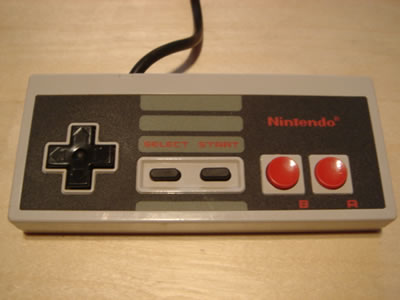
\includegraphics[width=4.5cm]{pics/nintendo.png}
\caption{The traditional Nintendo game controller.}
\label{fig:oldgamestick}
\end{figure}

Figure~\ref{fig:gamescreen} shows the 
screenshots of the famous 
Nintendo game \emph{Breakout}. In Figure~\ref{fig:gamescreen} (a), 
the paddle can only move horizontally along a predetermined line at a 
constant speed. Though it would be easy to implement the 
functionality to allow the paddle to move up and down, it 
will not be trivial to implement \emph{rotation} and \emph{varying speed} 
of the paddle while staying user-friendly, as shown 
in Figure~\ref{fig:gamescreen} (b).


Even with the advanced game controllers today, as shown in 
Figure~\ref{fig:newgamestick}, which have enough buttons 
and levers for different control commands, the implementation 
of \emph{rotation} and \emph{varying speed} can hardly be very 
intuitive. Even worse, it would be difficult for the players to 
manage all the buttons at the same time (Especially for real-time 
games). This may be one of the major reasons why many of today's 
video games are not so accessible to diverse groups of players.

\begin{figure}[h]
\centering
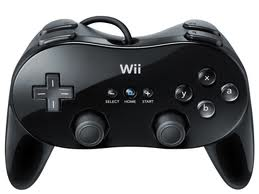
\includegraphics[width=5cm]{pics/stick.png}
\caption{The latest Nintendo game controller.}
\label{fig:newgamestick}
\end{figure}


\section{Visual Breakout}
Our project \emph{Visual Breakout} aims to use 
visual interface, espeically bare-hand gesture, to break 
through these limitations of Nintendo controllers. 

It would be very intuitive to use the position, 
angle and moving speed of the hand to represent 
the position, angle and speed of the paddle in 
breakout as shown in Figure~\ref{fig:gamescreen} (b). 
We will allow the paddle 
to travel to any positions in the game window if 
it does not overlap with other objects.

\begin{figure}[h]
\centering
\begin{tabular}{cc}
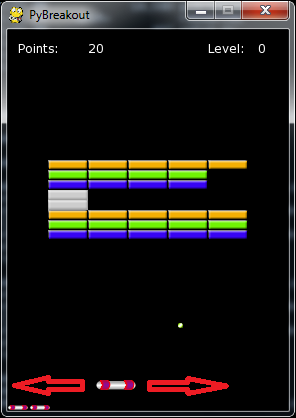
\includegraphics[width=4cm]{pics/horizontal.png} &
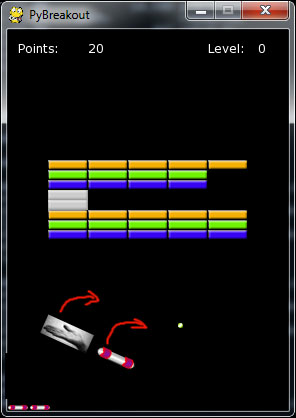
\includegraphics[width=4cm]{pics/tilt.png} \\
(a) &
(b)  
\end{tabular}
\caption{Screenshots of \emph{Breakout}. (a) Original design. 
the paddle can only move along with a predefined horizon. 
(b) Our new design. The paddle can tilt according to the rotation 
of the hand of the player.}
\label{fig:gamescreen}
\end{figure}

With this substantial change, new features are easy to be designed while the 
difficulty of playing the game must be re-balanced. Following is 
a list of new features we plan to implement.

\paragraph{Basic features}
\begin{itemize}
	\item Use hand movement to control the paddle position. The moving speed of the paddle is constant (as this basic feature) no matter how fast the hand is moving. The paddle can go any directions.
	\item Use the rotation of hand to control the orientation of the paddle. The orientation of the paddle will be at constant speed.
	\item Physical simulation of the bouncing angle of the ball. The original breakout does not follow physical laws to determine re-bounce angle of the balls. With allowing rotation of the paddle, this feature would be necessary. 
\end{itemize}
\paragraph{Optional features}
\begin{itemize}
	\item Variable speed of moving and rotation. The moving speed of hand should be mapped to a reasonable speed of the paddle (instead of simply proportionally.)
	\item Variable hit strength. The speed of the ball after collision is determined by the speeds and mass of both parts of the collision.
	\item Bricks which need multiple hits can be broken with a powerful hit. The power of the hit is determined by the speed of the ball.
	\item \emph{Buffered collision control}. This would be an advanced technique of the game. Players can slow down the ball by moving the paddle in the same direction of the moving ball at the moment when the ball is nearly colliding the paddle, just like technique soccer players use to stop the football. 
\end{itemize}

We also list some possible risks and difficulties that we may encounter:
\paragraph{Risks}
\begin{itemize}
	\item Environment impact on hand gesture detection.
	\item Hand gesture limitation. (Human hands are only comfortable to rotate steadily within small range of angle)
	\item Speed registration of the hand and the paddle. (the paddle must move continuously and cannot be too fast)
	\item Game difficulty balance. (For example, to allow the ball to escape from any side of the screen)
\end{itemize}
\section*{Appendix}
\appendix
\section{System dependency and external packages}
Instead of implementing the game from scratch, our implementation 
will base on an open source project published at: 
http://www.pygame.org/projects/20/314/?release\_id=501. We will 
focus the part of the gesture detection and translation, and the 
features with changes come with them.

Here are the list of packages that this system relies on:
\begin{itemize}
	\item Python 2.5.1
	\item pygame 1.7.1
	\item OpenCV 2.1
	\item Numpy 1.5.1
\end{itemize}

\section{Division of work}
Our system is composed of frontend computer vision modules, and the backend 
game control, response and rendering modules. Basically, Jie Huang will focus 
on the frontend, and Shao-Chuan Wang will focus on the backend. If 
someone is more overloaded, some tasks will be migrated to the other 
person.
{\small
\bibliographystyle{ieee}
\bibliography{egbib}
}


\end{document}
